\chapter{Measuring error on feature effects}
\label{chap:AssALE}

This chapter is dedicated to benchmarking the performance of various global explainable feature effect techniques under diverse data dependency scenarios, directly addressing RQ1. In addition to comparing these techniques, this work contributes to the existing literature by introducing a novel metric. This metric quantifies the degree of deviation of the explained feature effects from their true values. The introductory section establishes the significance and relevance of this chapter's contributions within the broader context of existing literature. Key concepts related to the contributions are defined, followed by a description of the benchmarking methodology employed. The chapter then presents and summarizes the experimental results, highlighting their role in addressing RQ1 and their impact on the field of \gls{XAI}

\begin{center}
  \fbox{
    \parbox{0.8\textwidth}{RQ1 - How do widely used feature effects techniques compare with ALE in accurately identifying true feature effects considering different inter-data dependencies?
    }
  }
\end{center}


\section{Introduction}

The global model explainability can be treated as a problem that entails the process of discerning, on average, how alterations in an input variable influence the model's predictions. In the case of linear models, the constant effects of features allow the attribution of feature contribution to be easily quantified using point estimates and variances of the model's parameters, which are essentially the estimated coefficient scores \cite{TrevorHastieRobertTibshirani2014AssessmentSelection}. Conversely, \gls{ML} models, which may encapsulate non-linear relationships, necessitate a more nuanced understanding of the intricate associations between the variables of interest and the target variable. While scores are still paramount to reporting the relevance of features in \gls{ML} for many tasks, more detailed visual representations to illustrate the behavior of the relationships between the feature of interest and the target can produce better communication about the whole feature behavior.

Several propositions have been made to alleviate the independence assumptions of some model feature effects explainers. These propositions often rely on the use of conditional instead of marginal distribution of features to avoid extrapolating the confinements of data relationships. Despite these advancements, the literature still lacks comprehensive analyses regarding the extent to which different strategies to handle data relationships affect explanations of feature effects \cite{Molnar2022GeneralModels}. Prior works have predominantly relied on theoretical discourse or visual demonstrations \cite{Apley2020VisualizingModels, Gkolemis2022DALE:Explanations, Gkolemis2023RHALE:Effects, Mangalathu2022Machine-learningSystems, Bakhshi2021UtilizingModels}, akin to the illustration in Figures \ref{fig:extrapolation_lr} and \ref{fig:extrapolation_rf}, to elucidate how explanations diverge when the actual data relationships are preserved during the computation of explanations and when not. Introducing a quantitative aspect would enhance the flexibility of this comparison framework, making it adaptable for future benchmarks. 

In a quantitative comparison akin to the current study, \cite{Molnar2023Model-agnosticApproach} evaluated model fidelity. The model fidelity concerns the difference between the predictions of the \gls{ML} model and the explanation method. The authors capture the overall difference in the model prediction and the prediction of the partial function when employed by the \gls{PD} plots and when deployed by \gls{ALE} plots. These differences were next averaged across all data points and features. The author found similar results when comparing model fidelity to \gls{PD} and \gls{ALE}.

Other work \cite{Gkolemis2022DALE:Explanations} compared the accuracy of \gls{ALE} and a version of a more computationally efficient ALE to recover the known true feature effects. The authors use the \gls{NMSE} to compare the computed partial functions and the true feature effects. The \gls{NMSE} is based on the expected value of the computed functions divided by their variance. 

Distinct from \cite{Molnar2023Model-agnosticApproach}, this study will assess the computed feature effects against the theoretically defined true feature effects in controlled experiments where the data generating functions are known. This is important since even a predictive model with explanations closely aligned to the model could, paradoxically, deviate significantly from the actual data-generating process \cite{Fisher2018AllSimultaneously, Slack2020FoolingSHAP}.  Such a comparison offers a more robust methodology for determining whether the model's explanations are more consistent with the actual data or the model's intrinsic structure. 

Moreover, different from both \cite{Molnar2023Model-agnosticApproach} and \cite{Gkolemis2022DALE:Explanations}, this study will individually evaluate the entire range of the explained feature, potentially uncovering a more nuanced understanding of discrepancies between explainable models. Unlike \gls{NMSE} from \cite{Gkolemis2022DALE:Explanations}, which disproportionately emphasizes larger errors, the \gls{ABX} proposed on this chapter, which is described bellow, uniformly accounts for all deviations across the feature's range, providing a more balanced evaluation and a more realistic assessment of a technique's accuracy. Finally, to the best of our knowledge, this study is the first to incorporate \gls{SHAP} global explanations into such a benchmark.


\subsection{The extrapolation problem}

One commonly utilized framework in the field of \gls{XAI} is based on post\-hoc analysis and frequently involves the processes of sampling a subset of data, intervening on the data, getting model predictions using the fitted model, and subsequently aggregating them to quantify changes in outputs and produce model explanations \cite{Scholbeck2020SamplingInterpretations}. While there are numerous variations in how each step is executed, a critical step within this framework is the intervention step.

Interventions involve altering the values of the features of interests on the \textit{ceteris paribus} reasoning. When the interventions are beyond the confines of the actual conditional distribution, it becomes possible to generate unlikely data points. Such circumstances compel the model to make predictions in regions where it was not trained, potentially yielding unexpected results. Consequently, changes in the model's outputs can lead to unrealistic model explanations regarding the true data-generating process. This issue would not be a concern if the goal were to understand the function's behavior itself, but it certainly presents difficulties when the aim is to uncover the potential data-generating process.

\gls{XAI}  techniques that modify features based on their values concerning the entire dataset pose a significant challenge when explaining non-additive functions. These model-agnostic techniques inherently assume feature independence and intervene by using the marginal distribution of a feature, which can lead to misinterpretations when this intervention extrapolates outside of the training data's scope. The root of this issue lies not in the predictive models themselves but rather in the assumptions that these interpretive techniques make about the underlying data. In a hypothetical situation where it is possible to assume that the feature of interest is independent of others, extrapolation would not be a concern. Otherwise, the model's outputs could even be interpreted as the causal effect of the potential intervention of \(X\) on \(y\) \cite{Zhao2021CausalModels}. However, this is often not the case in real-world scenarios. 

Based on \cite{molnar2019}, Figure \ref{fig:extrapolation_lr} illustrates a simulation of this issue. The figure provides explanations for the function $f$ for each variable in $X = {x_1, x_2}$ regarding their predictive role in $Y$ involving four different techniques: \gls{PD} plots and \gls{SHAP}, which tend to extrapolate by utilizing the marginal distribution of the feature of interest for intervention, and \gls{ALE} and \gls{ME} plots, which do not. 

To simulate the unexpected behavior of $f$ when predicting outside of the training data envelope - thus violating conditional relationships accessing regions of the input space not covered by the training data - $f$ was artificially constrained to make incorrect predictions within this region. Specifically, it was programmed to consistently predict a constant value in a region of the data distribution that does not exist, illustrating a potential problem when the function is used to predict beyond the bounds of its training data. The predictive function was adjusted to make predictions as follows:

$\($f(x_1, x_2) =$ 
\begin{cases} 
2 & \text{if } x_1 > 0.7 \text{ and } x_2 < 0.3 \\
x_1 + x_2 & \text{otherwise}
\end{cases}



\begin{figure}[ht!]
\centering
  \fcolorbox{gray}{white}{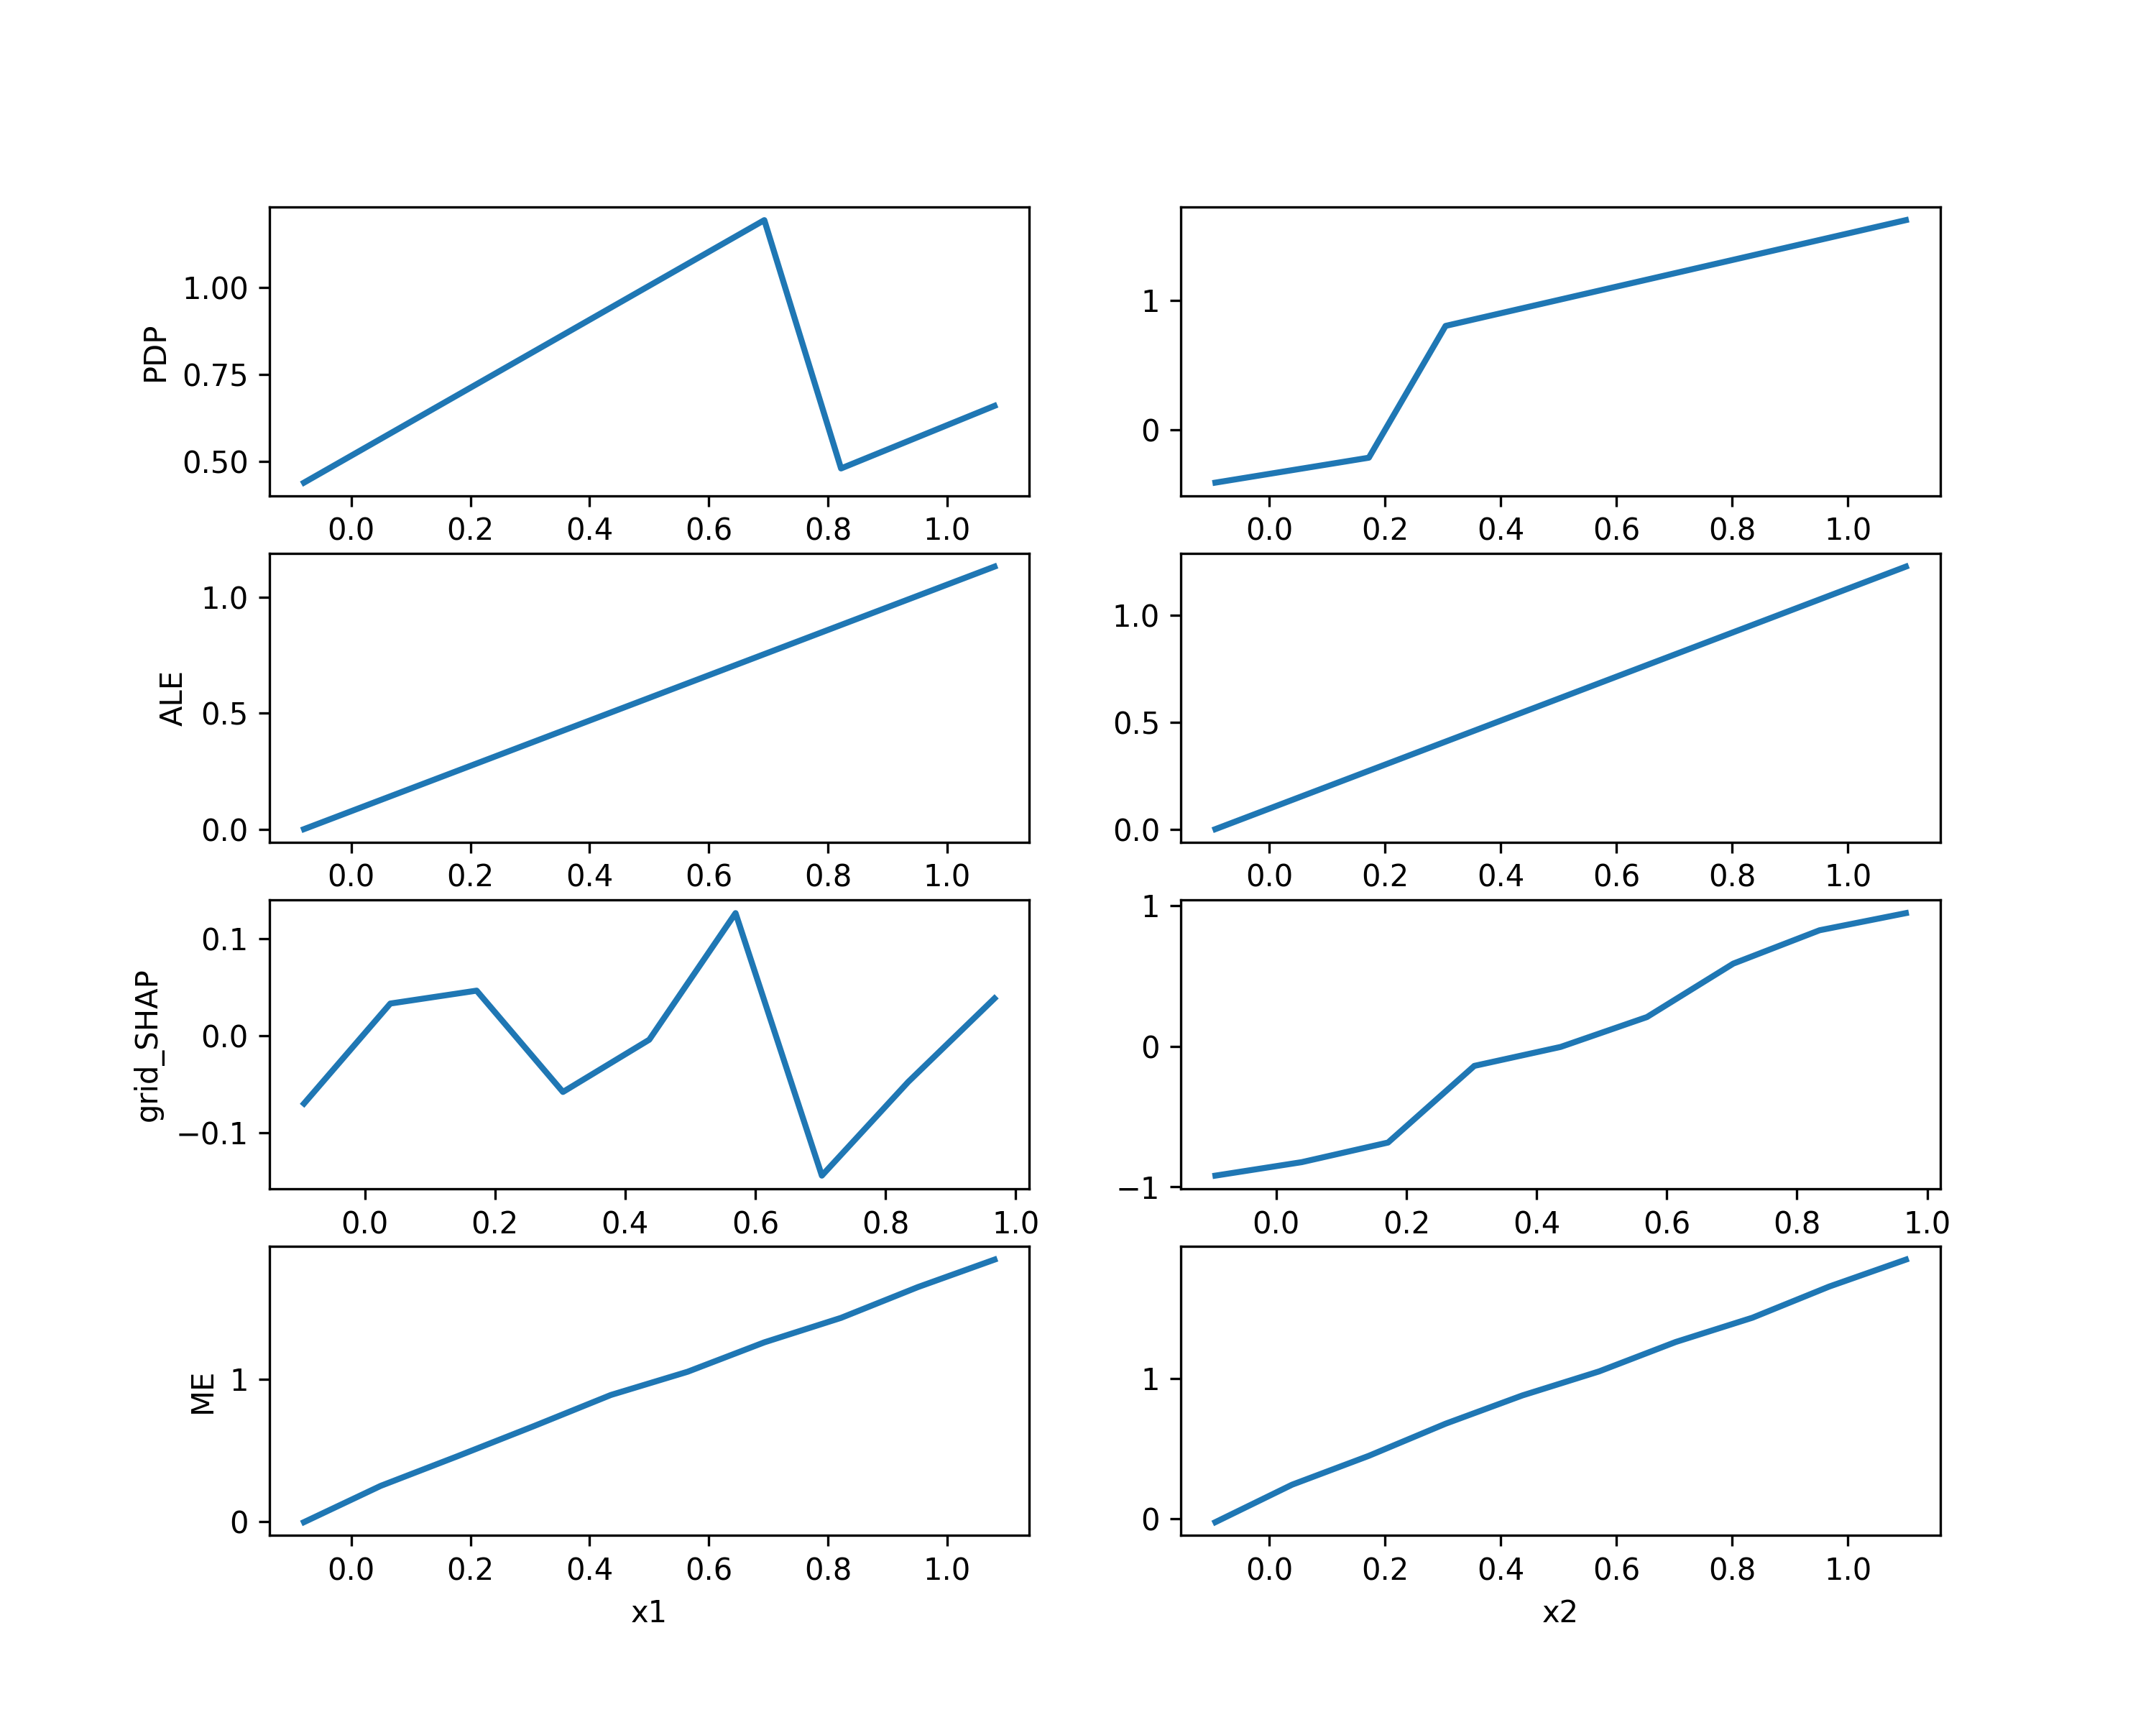
\includegraphics[width=0.98\textwidth]{images/extrapolation/extrapolation_lr.png}}
  \caption{Explanation of the customized linear regression model for predicting a constant in a region beyond the training data bounds. The dataset was generated using the function \(f(x_1,x_2) = Y = x_1 + x_2\)}
    \label{fig:extrapolation_lr}
\end{figure}

Notably, \gls{PD} plot and \gls{SHAP} (for \(x_1\)) demonstrate greater sensitivity to the artificial bias introduced in the model. Conversely, \gls{ME} and \gls{ALE} plots remain robust in this same scenario, consistently revealing the true linear effects of both $x_1$ and $x_2$ as defined in the function \(f\).  In other words, \gls{PD} plot and  closely align with the model (predict a constant in the region where $x_1 > 0.7$ and $x_2 <0.3 $) but move away from the data-generating function. While this isn't problematic per se, as the \gls{PD} plot and \gls{SHAP} approximate the model's behavior, they can pose challenges when they are used to explain the roles of highly correlated features due to their susceptibility to extrapolation.


\subsection{Importance of interventional distribution}
\label{intervention}

While preserving the conditional distribution seems to be the right way to explain the global behavior of dependent features, there is another important aspect: the use of interventional instead of observational expectation. Just keeping the conditional distribution without using an unrealistic combination of data points is not enough to recover the right effects of dependent variables. The need for interventional expectation in model-agnostic explainable techniques instead of observational has been already formally discussed in \cite{Janzing2020FeatureProblem} as a recommendation to researchers who intend to extend the \gls{SHAP} technique. 

The concept of interventional expectation was first introduced in the causality literature \cite{Pearl1993BayesianIntervention} aiming to elucidate the effect of manipulating a specific feature within a hypothetical scenario. In this context, the manipulation entails substituting the value of$x_1$ for that feature, while holding the values of all other features constant. Specifically, given $X={x_1, x_2,...,x_n}$ a function $f(X)$ that predict $Y$, the interventional expectation regarding $x_1$ is defined by using the "do-operator" through \(E[Y | do(X_{1} = x_{1})]\). The "do-operator" defined by Pearl allows researchers to formalize and analyze the causal effect of setting a variable \(X\) to a particular value \(x\), effectively simulating an intervention in the system.  

In the traditional statistical literature, the use of \gls{ME} plots have long been proposed as one of the reliable way to interpret models in place of the coefficients \cite{long1997regression}. The \gls{ME} corresponds to the average differences in the outcome when the features partially change from one specified value to another. The \gls{ME} uses the observed conditional distribution and does not extrapolate the joint distribution present in the data. However, \gls{ME} is not able to differentiate the effects of correlated variables as the changes in the outputs are computed while changing all dependent variables in tandem using the observed distribution.

To illustrate how the use of observed distribution in a highly correlated scenario fails to recover the individual role of features, Figure \ref{fig:extrapolation_rf} shows the same issue as Figure \ref{fig:extrapolation_lr}, where the predictive function has unexpected results when predicting outside of the training data envelope. Now, the output $y$ is defined by $f(x) = x_1 + x_2^3$ and the data was fitted by the non-linear random forest algorithm, which might be able to detect the new cubic effect of $x_2$. In this case, differently from \gls{ALE} plot that correctly traces a linear effect to $x_1$ and an exponential effect to $x_2$ , \gls{ME} recovered the same effects for both variables. 

The tension between the use of observational and interventional distribution has also been discussed around the implementation of \gls{SHAP}. Some authors argue that the use of observed expectation can attribute importance to irrelevant features \cite{Janzing2020FeatureProblem, Sundararajan2020TheExplanation} while using interventional can lead to extrapolation issues. In \cite{Chen2020TrueData}, the authors suggest that there is no correct choice for this value function. Instead, the crux of the interpretation hinges on whether the aim is fidelity to the model or alignment with the data.

Within this context, \gls{ALE} technique emerges as a suitable tool for global explanations of feature effects to real applications, where variables are not independent. \gls{ALE} has a good balance of the tradeoff of being true to the model and true to the data, as it uses the interventional conditional expectation. In other words, \gls{ALE} takes advantage of interventions to break variable dependencies while adhering to the data joint distribution when computing effects by parts of the data.

\begin{figure}[ht!]
\centering
  \fcolorbox{gray}{white}{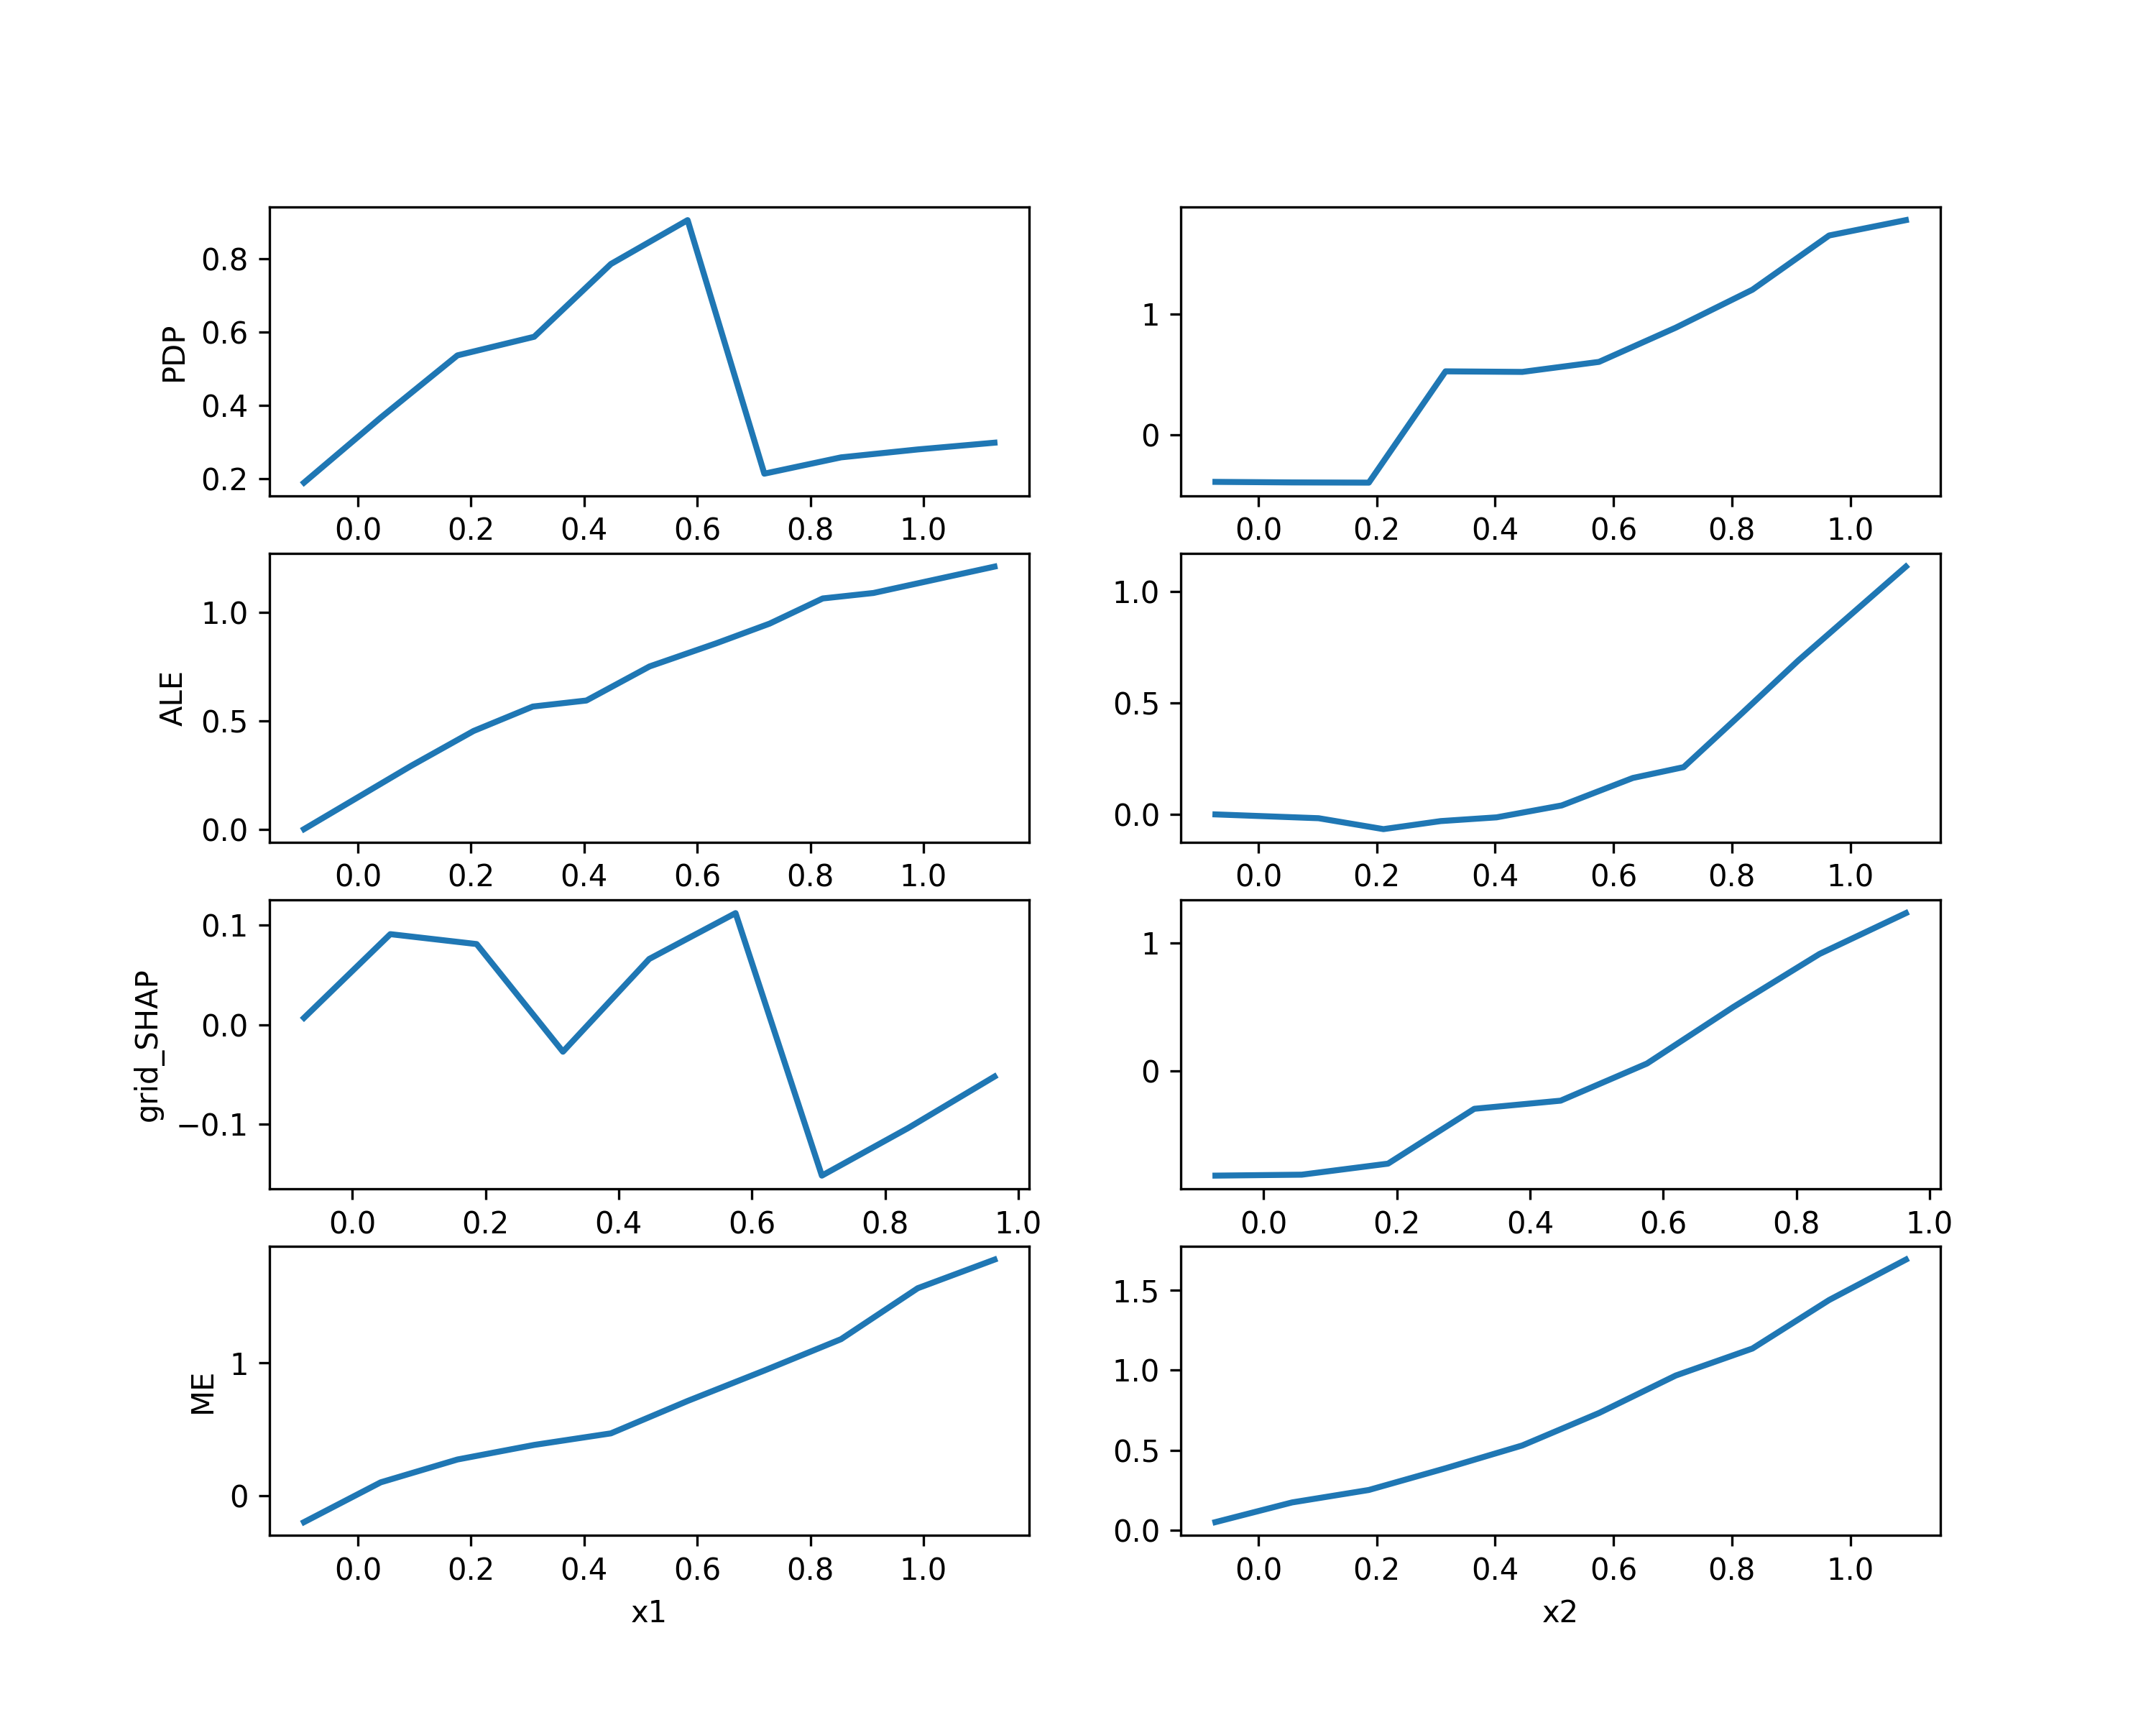
\includegraphics[width=0.98\textwidth]{images/extrapolation/extrapolation_rf.png}}
  \caption{Explanation of the customized random forest model for predicting a constant in a region beyond the training data bounds. The dataset was generated using the function $y = x_1 + x_2^3$}
    \label{fig:extrapolation_rf}
\end{figure}






